\section{Introduction}
Unmanned aerial vehicles (UAVs) has gained significant attention in recent years due to their potential applications in various fields, including surveillance, search and rescue operations, and infrastructure inspection~\cite{8682048,9990164}. One crucial aspect of UAV operations is their ability to navigate and maintain formations effectively, especially in complex environments with obstacles. The formation control of multiple UAVs thus plays a vital role in achieving coordination and efficient mission execution~\cite{Anderson,9990236}.

Formation control in multi-robot systems refers to the coordination and control strategies used to form, maintain, and transform formations among a group of robots~\cite{736776,Balch2000}. In scenarios with dense obstacles or narrow spaces, UAV formations need to adapt and reconfigure their shape to navigate through or around obstacles~\cite{7487747,Dang2019,8843165}, as described in Figure~\ref{fig:idea}. This self-reconfigurable capability enables the UAVs to overcome challenging terrain, narrow passages, or complex structures, thereby enhancing their maneuverability and overall mission success. One commonly adopted formation shape is the V-shape configuration, which offers advantages in terms of stability, visibility, and aerodynamic efficiency~\cite{Dang2019,Mirzaeinia2019}. In~\cite{Dang2019}, a formation control algorithm is proposed for multi-UAV systems where the UAVs autonomously adjust their positions within a V-shape to avoid collisions with obstacles. In~\cite{8793765}, a splitting and merging algorithm is proposed for multi-robot formations in environments presented by static and dynamic obstacles. The work in~\cite{8594438} presents a switching strategy of a region-based shape controller for a swarm of robots to deal with the obstacle-avoidance problem in complex environments. 

\begin{figure}
    \centering
    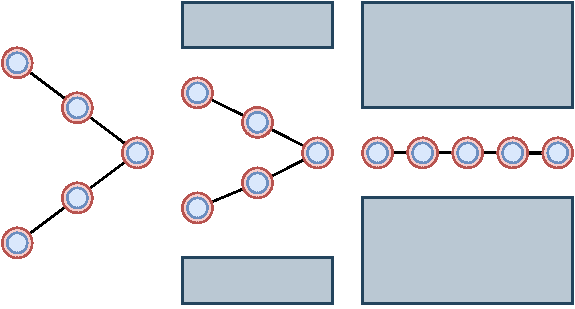
\includegraphics[width=0.6\textwidth]{paper1/images/idea.pdf}
    \caption{The self-reconfigurable V-shape formation can adjust its shape and navigate through narrow passages.}
    \label{fig:idea}
\end{figure}

Recently, advancements in path planning and obstacle avoidance techniques have contributed to the development of self-reconfigurable formation control algorithms. In \cite{8843165}, the angle-encoded particle swarm optimization algorithm is developed for the formation of multiple UAVs used in vision-based inspection of infrastructure. By incorporating constraints related to flight safety and visual inspection, the path and formation can be combined to provide trajectory and velocity profiles for each UAV. The work in \cite{FENG2022} developed a novel optimization method for multi-UAV formation to achieve rapid and accurate reconfiguration under random attacks. In \cite{Gao2022}, multi-UAV reconfiguration problems are modeled as an optimal problem with task assignment and control optimization. However, the focus of their work was on maintaining a fixed formation shape rather than self-reconfiguration in the presence of obstacles.

% \hl{Formation control in environments with obstacles and narrow passages presents challenges in obstacle avoidance, passing through constrained spaces, and so on \cite{Huang2019,Saska2020}. To address these challenges, building a self-reconfiguration formation control strategy is crucial. Such a strategy ensures robustness, adaptability, and efficient navigation, allowing the formation to autonomously adjust its shape to navigate through narrow gaps and avoid obstacles without external intervention. It enhances safety, and mission continuity, making autonomous multi-agent systems more capable and effective in complex and dynamic environments for various applications. Although research efforts have been made in the area of self-reconfigurable formation control, limited work has specifically addressed the challenges of self-reconfigurable formations in large obstacles and narrow environments. }

In this work, we propose a self-reconfigurable V-shape formation control algorithm for multiple UAVs operating in narrow space where the formation cannot maintain its initial shape when moving through this space. The algorithm allows the UAVs to form, maintain and reconfigure the desired V-shape formation by expanding/shrinking its two V-wings to avoid collisions with obstacles and maintain distances among the UAVs. According to the proposed design of distributed behaviors, the V-shape formations can open/close wings or merge into a straight line. Based on it, the UAVs can navigate through narrow passages, bypass obstacles, and optimize their trajectory in accordance to environmental conditions. The main contributions of our work are twofold: (i) develop a self-reconfiguration strategy that can adjust its shape in narrow space environments; and (ii) propose reconfiguration behaviors that navigate UAVs and maintain their shape.

% The remaining sections of this paper are structured as follows. Section \ref{sec:0design} describes the design of the V-shape formation. Section \ref{sec:0control} presents our implementation of the behavior-based controller. Section \ref{sec:0result} shows simulation results. Our paper ends with conclusions drawn in Section \ref{sec:0conclusion}.